\subsection{Privilege Level Switching}
\label{sec:privilege_switches}

Applications software needs a method to invoke the kernel, because it cannot
directly perform privileged operations, such as network or disk I/O. At the
same time, ring 3 software cannot be offered the ability to jump arbitrarily
into kernel code, as that would compromise the kernel's ability to isolate
applications and enforce security invariants.\footnote{For example, when an
application wishes to write a file to the disk, the kernel must check if the
application's user has access to that file. If the ring 3 code could perform
an arbitrary jump in kernel space, it would be able to skip the access check.}
Therefore, the processor has designated methods for switching privilege levels,
which protect the integrity of the more privileged software.

This section describes the privilege switching mechanisms that impact the SGX
design, summarized in Figure~\ref{fig:cpu_ring_switch}. Also, understanding the
considerations behind privilege switching is useful when analyzing SGX, because
the process of calling code inside an enclave is similar to switching privilege
levels, as an enclave's code must be able to enforce its own security
invariants, just like an OS kernel.


\subsubsection{System Calls}
\label{sec:syscalls}

% Fast System Calls in 64-Bit Mode: SDM S 5.8.8

\begin{figure}[hbt]
  \center{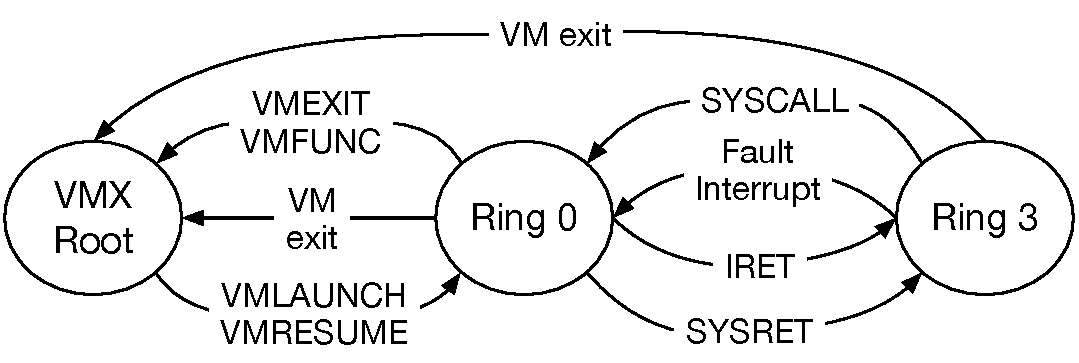
\includegraphics[width=85mm]{figures/cpu_ring_switch.pdf}}
  \caption{
    Modern privilege switching methods in the 64-bit Intel architecture.
  }
  \label{fig:cpu_ring_switch}
\end{figure}

On modern processors, application software uses the \texttt{SYSCALL}
instruction to invoke ring 0 code, and the kernel uses \texttt{SYSRET} to
switch the privilege level back to ring 3. \texttt{SYSCALL} jumps into a
predefined kernel location, which is specified by writing to a pair of
architectural MSRs (\S~\ref{sec:address_spaces}).  MSRs can only be read or
written by ring 0 code, so application software cannot modify
\texttt{SYSCALL}'s MSRs and abuse the \texttt{SYSCALL} instruction to execute
arbitrary kernel code. The \texttt{SYSRET} instruction switches back to ring 3
and jumps to the address in RCX, which is set by the \texttt{SYSCALL}
instruction. The \texttt{SYSCALL} / \texttt{SYSRET} pair is optimized for speed
by avoiding memory accesses. The design can get away without referencing a
stack because kernel calls are not recursive.


\subsubsection{Faults}
\label{sec:faults}

% Interrupt and Exception Handling: SDM S 6.1, S 6.2
% Access Rights: SDM S 4.6
% Page-Fault Exceptions: SDM S 4.7

The processor also performs a switch from ring 3 to ring 0 when a \textit{
hardware exception} occurs while executing application code. Some exceptions
indicate bugs in the application, whereas other exceptions require kernel
action. A \textit{general protection fault} (\#GP) occurs when software
attempts to perform a disallowed action, such as setting the CR3 register from
ring 3. A \textit{page fault} (\#PF) occurs when address translation encounters
a page table entry whose P flag is 0, or attempting to use a page in a way
inconsistent with the access bits in its page table entry, for example
accessing a page whose S bit is set from ring 3.

% Interrupt Descriptor Table (IDT): SDM S 6.10

When a hardware exception occurs in application code, the CPU performs a ring
switch, and calls the corresponding \textit{exception handler}. For example,
the \#GP handler typically terminates the application's process, while the \#PF
handler reads the swapped out page back into RAM and resumes the application's
execution.

The exception handlers are a part of the OS kernel, and their locations are
specified in the first 32 entries of the Interrupt Descriptor Table (IDT),
whose structure is shown in Table~\ref{fig:idt_entry}. The IDT's physical
address is stored in the IDTR register, which can only be accessed by ring 0
code. Kernels protect the IDT memory using page tables, so that ring 3 software
cannot access it.

\begin{table}[hbt]
  \center{\begin{tabular}{| l | r |}
  \hline
  \textbf{Field} & \textbf{Bits} \\
  \hline
  Handler RIP & 64 \\
  \hline
  Handler CS & 16 \\
  \hline
  Interrupt Stack Table (IST) index & 3 \\
  \hline
  \end{tabular}}
  \caption{
    The essential fields of an IDT entry in 64-bit mode. Each entry points to a
    hardware exception or interrupt handler.
  }
  \label{fig:idt_entry}
\end{table}

Each IDT entry has a 3-bit index pointing into the Interrupt Stack Table (IST),
which is an array of 8 stack pointers stored in the TSS described in
\S~\ref{sec:segments}.

% 64-Bit Mode Stack Frame: SDM S 6.14.2
% IRET in IA-32e Mode: SDM S 6.14.3
% Stack Switching in IA-32e Mode: SDM S 6.14.4
% Interrupt Stack Table: SDM S 6.14.5

When a hardware exception occurs, the execution state may be corrupted, and the
current stack cannot be relied on. Therefore, the CPU first uses the handler's
IDT entry to set up a known good stack. SS is loaded with a null descriptor,
and RSP is set to the IST value pointed by the IDT entry. After switching to a
reliable stack, the CPU pushes the snapshot in Table~\ref{fig:fault_stack} on
the stack, then loads the IDT entry's values into the CS and RIP registers,
which trigger the execution of the exception handler.

\begin{table}[hbt]
  \center{\begin{tabular}{| l | r |}
  \hline
  \textbf{Field} & \textbf{Bits} \\
  \hline
  Exception SS & 64 \\
  \hline
  Exception RSP & 64 \\
  \hline
  RFLAGS & 64 \\
  \hline
  Exception CS & 64 \\
  \hline
  Exception RIP & 64 \\
  \hline
  Exception code & 64 \\
  \hline
  \end{tabular}}
  \caption{
    The snapshot pushed on the handler's stack when a hardware exception
    occurs. IRET restores registers from this snapshot.
  }
  \label{fig:fault_stack}
\end{table}

After the exception handler completes, it uses the \texttt{IRET} (interrupt
return) instruction to load the registers from the on-stack snapshot and switch
back to ring 3.

The Intel architecture gives the fault handler complete control over the parts
of the execution context not listed in Table~\ref{fig:fault_stack}. This
privilege is used by some handlers (e.g., \#GP) to perform context switches
(\S~\ref{sec:registers}) after a process is terminated due to a bug. However,
in the SGX threat model, system software is not trusted, and giving it access
to an enclave's execution context would expose potentially sensitive
information, and present an opportunity to compromise the enclave's integrity.
Therefore, SGX cannot use the current fault handling process, and must modify
it.


\subsubsection{VMX Privilege Level Switching}
\label{sec:vmx}

% Life Cycle of VMM Software: SDM S 23.4
% Virtual-Machine Control Structure: SDM S 23.5

Intel systems that take advantage of the hardware virtualization support to run
multiple operating systems at the same time use a hypervisor that manages the
VMs. The hypervisor creates a \textit{Virtual Machine Control Structure} (VMCS)
for each operating system instance that it wishes to run, and assigns a VM to a
logical processor by executing the \texttt{VMENTER} instruction.

% VM Exists: SDM S 27
% EP{T_Induced VM Exits: SDM S 28.2.3

When a logical processor encounters a fault that must be handled by the
hypervisor, the logical processor performs a VM exit. For example, if the
address translation process encounters an EPT entry with the P flag set to 0,
the CPU performs a VM exit, and the hypervisor has an opportunity to bring the
page into RAM.

The VMCS shows a great application of the encapsulation principle
\cite{liskov1974adt}, which is generally used in high-level software, to
computer architecture. The Intel architecture specifies that each VMCS resides
in DRAM and is 4~KB in size. However, the architecture does not specify the
VMCS format, and instead requires the hypervisor to interact with the VMCS via
CPU instructions such as \texttt{VMREAD} and \texttt{VMWRITE}.

This approach allows Intel to add VMX features that require VMCS format
changes, without the burden of having to maintain backwards compatibility.
This is no small feat, given that huge amounts of complexity in the Intel
architecture were introduced due to compatibility requirements.
